\subsection{Tiles à la Google Maps}
Maptiler bietet auf ihrer Webseite\footnote{\url{http://www.maptiler.org/google-maps-coordinates-tile-bounds-projection/}} ein Python Script an, welches den Umgang mit Tiles stark vereinfacht. Unter anderem wir die Umrechnung von Meter zu Latitude/Longitude, Meter zu Pixel und für unsere arbeit noch wichtig, Tiles zu QuadTree\footnote{\url{https://msdn.microsoft.com/en-us/library/bb259689.aspx}} (Bing Format für Tiles).

\begin{figure}[H]
\centering
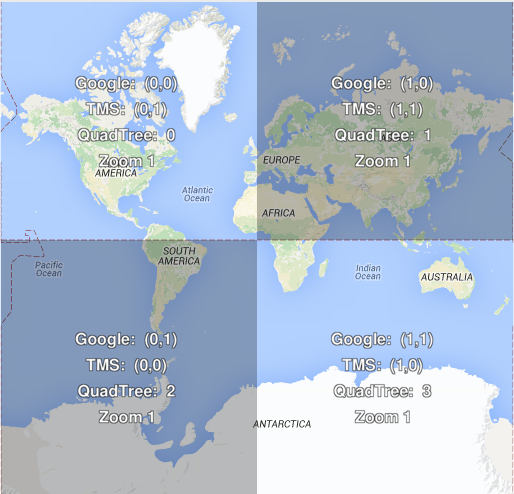
\includegraphics[width=0.5\textwidth]{images/tiles_a_la_google.png}
\caption[Tiles à la Google Maps]{Tiles à la Google Maps}
\end{figure}

\subsubsection{QuadKey}
Die Quadkeys von Bing Maps bauen sich folgendermassen auf:
\begin{figure}[H]
\centering
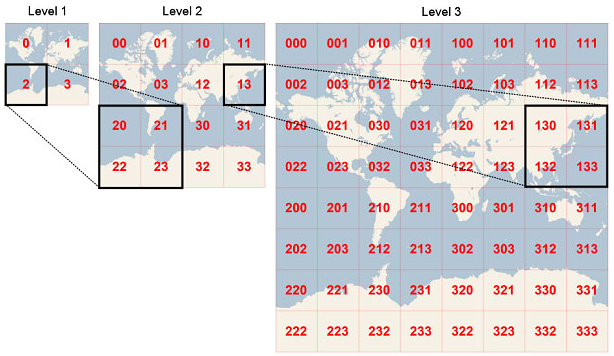
\includegraphics[width=\textwidth]{images/quadkey.png}
\caption[Tiles à la Google Maps]{Tiles à la Google Maps}
\end{figure}